\documentclass[12pt,a4paper]{scrartcl}
\usepackage[utf8]{inputenc}
\usepackage[ngerman]{babel}
\usepackage{amsmath}
\usepackage{amsfonts}
\usepackage{amssymb}
\usepackage{color}
\usepackage{graphicx}
\usepackage{listings}
\usepackage[left=2.5cm, right=2cm, top=2cm, bottom=2cm]{geometry}

\usepackage[hidelinks]{hyperref}
\usepackage{scrpage2}
\usepackage{csquotes}
\usepackage{subcaption}

%\usepackage{pdfpages}


\DeclareUnicodeCharacter{00A0}{ }

\pagestyle{scrheadings}


\linespread{1.5}
\setlength{\parindent}{0cm} % No paragraph indent


\newcommand{\q}[1]{``#1''}
\newcommand{\todo}[1]{\begin{Large}\textcolor{red}{$\Rightarrow ~$#1}\end{Large}}

\newcommand{\ant}[1]{\begin{Large}\textcolor{green}{$\Rightarrow ~$#1}\end{Large}}


\newcommand{\inmilestonetwo}{\vspace{0.75cm} \framebox[1.1\width]{
\begin{large}
\textcolor{red}{Die Dokumentation dieses Abschnittes ist für Milestone II vorgesehen.}
\end{large}}}



\begin{document}

% University Assignment Title Page 
% LaTeX Template
% Version 1.0 (27/12/12)
%
% This template has been downloaded from:
% http://www.LaTeXTemplates.com
%
% Original author:
% WikiBooks (http://en.wikibooks.org/wiki/LaTeX/Title_Creation)
%
% License:
% CC BY-NC-SA 3.0 (http://creativecommons.org/licenses/by-nc-sa/3.0/)
% 

\begin{titlepage}

\newcommand{\HRule}{\rule{\linewidth}{0.5mm}} % Defines a new command for the horizontal lines, change thickness here

\center % Center everything on the page
 
%----------------------------------------------------------------------------------------
%	HEADING SECTIONS
%----------------------------------------------------------------------------------------

\textsc{\LARGE Programmierprojekt}\\[1.5cm] % Name of your university/college
\textsc{\Large Alte Kantonsschule Aarau}\\[0.5cm] % Major heading such as course name
\textsc{\large}\\[0.5cm] % Minor heading such as course title

%----------------------------------------------------------------------------------------
%	TITLE SECTION
%----------------------------------------------------------------------------------------

\HRule \\[0.4cm]
{ \huge \bfseries Dokumentation: Spacetraveler}\\[0.4cm] % Title of your document
\HRule \\[1.5cm]
 
%----------------------------------------------------------------------------------------
%	AUTHOR SECTION
%----------------------------------------------------------------------------------------

\begin{minipage}{0.4\textwidth}
\begin{flushleft} \large
\emph{Autoren:}\\
Gabriel \textsc{Gavrilas}\\ % Your name\\
Patrick \textsc{Eigensatz}\\ % Your name\\
Jonas \textsc{Wahlen}\\ % Your name\\
\end{flushleft}
\end{minipage}
~
\begin{minipage}{0.4\textwidth}
\begin{flushright} \large
%\emph{Betreuer:} \\
%Dr. Martin \textsc{Jordi} % Supervisor's Name
\end{flushright}
\end{minipage}\\[2cm]

% If you don't want a supervisor, uncomment the two lines below and remove the section above
%\Large \emph{Author:}\\
%John \textsc{Smith}\\[3cm] % Your name

%----------------------------------------------------------------------------------------
%	DATE SECTION
%----------------------------------------------------------------------------------------

{\large Februar 2016}\\[2cm] % Date, change the \today to a set date if you want to be precise

%----------------------------------------------------------------------------------------
%	LOGO SECTION
%----------------------------------------------------------------------------------------

%\includegraphics[width=12cm]{img/titelbild.jpg}\\[1cm] % Include a department/university logo - this will require the graphicx package
 
%----------------------------------------------------------------------------------------

\vfill % Fill the rest of the page with whitespace

\end{titlepage}

\clearpage

\tableofcontents

\clearpage

\todo{Informationen / Beispielarbeit beachten!}

\section{Projektbeschreibung}
\subsection{Spielidee}
Ziel unseres Spieles ist es, dass der Spieler sein Raumschiff von einer Startposition im Level
zum Ziel bringt. Dazu eine kleine Story:
\begin{quote}
Der verrückte Wissenschaftler Prof. Lewinsky war mit seiner Rakete auf der Suche nach einem äusserst seltenen Element welches er zur Fertigung seiner Gravitationskanone benötigt. 
In einer weit entfernten Galaxie wurde er fündig. 
Beim Treibstoff hatte er sich jedoch verrechnet und stand nun ohne Antrieb am anderen Ende des Universums.
Glücklicherweise konnte er seine Gravitationskanone an Bord fertigstellen.
Deine Aufgabe ist es nun Prof. Lewinsky mithilfe der instabilen und ungetesteten Gravitationskanone nach Hause zu befördern. 
Dabei musst du auf die herumfliegenden Asteroiden achtgeben. 
Vor allem solltest du dich jedoch vor den abnormal kleinen Schwarzen Löchern in Acht nehmen, die nur in diesem Teil des Universums vorkommen und dich sofort anziehen, wenn du ihnen zu nahe kommst. 
Hilf dem hoffnungslosen Theoretiker nach Hause zu kommen!
\end{quote}

\subsection{Physik}
In unserem Spiel haben wir einige Elemente der Physik der realen Welt übernommen.
Dabei handelt es sich nur schon um Geschwindigkeit, Beschleunigung und Kräfte.
Dazu haben wir auch die Gravitation und den elastischen Stoss, als komplexere Vorgänge modelliert.
\subsubsection{Geschwindigkeit, Beschleunigung, Kraft}
Unser Spieler bewegt sich im Level.
Hier ist bereits die Sprache von Geschwindigkeit.
Zur Geschwindigkeit ist wohl keine Erklärung nötig.
Dazu kommt die Beschleunigung, die man als zeitliche Änderung der Geschwindigkeit auffassen kann.
Wichtig zu verstehen ist jedoch der Zusammenhang zwischen Kraft und Beschleunigung.
Um Kräfte zu berechnen nimmt man das Produkt aus Beschleunigung und Masse.
Also ist die Beschleunigung, wenn die Kraft bekannt ist, auch von dem Faktor Masse abhängig. ...

\subsection{Gravitation}
Unter Gravitation versteht man in der Physik, die Anziehungskraft, mit der sich Masse anzieht.
Bekannt ist uns die Gravitation von den Planeten und ihren Anziehungskräften.
Die Sonne zieht mit ihrer enormen Masse die Planeten an und die Planeten ziehen die Monde an.
Auf der Erde zeigt sich Gravitation als Schwerkraft, die uns am Boden hält.
Dies kommt davon, dass die Erde sehr viel grösser als wir ist.
Im Sonnensystem jedoch findet Gravitation zwischen Objekten ähnlicher Grösse statt.
Wenn sich ein Objekt einem anderen nähert gibt es drei Mögliche Auswirkungen.
\begin{enumerate}
\item Sie ziehen sich gegenseitig so an, dass sie miteinander kollidieren.
\item Sie sind schnell und lenken sich gegenseitig bei nahekommen einfach ab, entfernen sich danach jedoch zu weit um weiter Einfluss aufeinander zu bewirken.
\item 

\end{enumerate}


\subsection{Elastischer Stoss}
Im Spiel brauchen wir bei der Kollision der einzelnen Asteroiden und der Kollision mit der Wand das Prinzip des vollkommen elastischen Stosses. \\
In der realen Welt kommt es ständig zu Kollisionen, sei es ein Fuss, der auf einen Ball trifft, Billardkugeln die Kollidieren, oder zwei Autos bei einer Frontalkollision. 
Ständig stossen Objekte aufeinander. \\
Die Physik kennt verschiedene Arten solcher Stösse.
Unterschieden wird dabei, wie Energie übertragen wird.
Speziell im Bezug auf den Stoss sind das innere Energie und kinetische Energie.
Einfach gesagt unterscheidet man, ob sich Objekte bei einer Kollision verformen und/oder erhitzen, oder sie ihre Geschwindigkeit und Richtung ändern.\\
Die Extremfälle bilden also zum einen ein Stoss, bei dem Beide Objekte sofort still stehen und sich erwärmen oder deformieren.
Dies nennt man den vollkommen unelastischen Stoss.
Zum anderen ein Stoss, bei dem die Objekte keine Deformation oder Erwärmung erfahren, sondern eine Änderung der Geschwindigkeit und der Bewegungsrichtung stattfindet.
Dies nennt man den vollkommen elastischen Stoss.\\
Beide Fälle sind Idealfälle.
Sie kommen in der realen Welt nicht vor.
In unserem Spiel wollten wir einen beinahe vollkommen elastischen Stoss umsetzen.
\todo{langet da? wo selli da wege vektorfällig schriibe im andere teil denne?}
\ant{Jio, da wär gäbig...}




\section{Problemdefinition}
\subsection{Grundkriterien}
Wir haben uns folgende Grundkriterien gesetzt:
\begin{itemize}
\item Gravitation: Punkte, die den Spieler unterschiedlich stark gegen sich ziehen.
\item Der Spieler ist ein Raumschiff.
\item Der Spieler befindet sich in einem Raum fernab von jeder anderen Kraftquelle ausserhalb des Levels.
\item Der Spieler bewegt sich durch dieses Level mithilfe von  einem Gravitationspunkt, den er platzieren und entfernen kann; Er kann sich also \q{in eine Richtung ziehen lassen}
\item Das Level ist beschränkt, hat also einen Start und ein Ziel
\item Es gibt Wände, die den Raum beschränken.
\end{itemize}

\subsection{Zusatzkriterien}
Als Zusatzkriterien setzen wir uns weiter:
\begin{itemize}
\item Gegner und/oder Hindernisse (= Objekte bei deren Kollision der Spieler stirbt) z.B: Asteroiden die sich frei bewegen, oder sehr starke Gravitationszentren, die den Spieler gegen ein Objekt ziehen und so eine Kollision auslösen.
\item Gameover-Grafik, die angezeigt wird, wenn der Spieler stirbt oder die Zeit abläuft.
\item Es besteht eine kleine Reibung, die den Spieler leicht abbremst.
\item Zeitliche Beschränkung (z.B: 2min, wenn Zeit = 0, ist das Spiel zu Ende)
\item Startmenu und Spielanleitung
\end{itemize}




\section{Anforderungsanalyse}
% maximal 2 sätze, in java realisierbar
Das Programm lässt sich mitsamt seinen Anforderungen vollständig in Java implementieren.
Es werden auf Soft-/Hardwareebene keine weiteren Anforderungen gestellt, als ein einfacher Computer mit
Maus und funktionierender JRE.


\section{Spezifikation}
\subsection{Use Cases}
\todo{Weitere Usecases folgen in Milestone II}

\subsubsection{spaceObject}
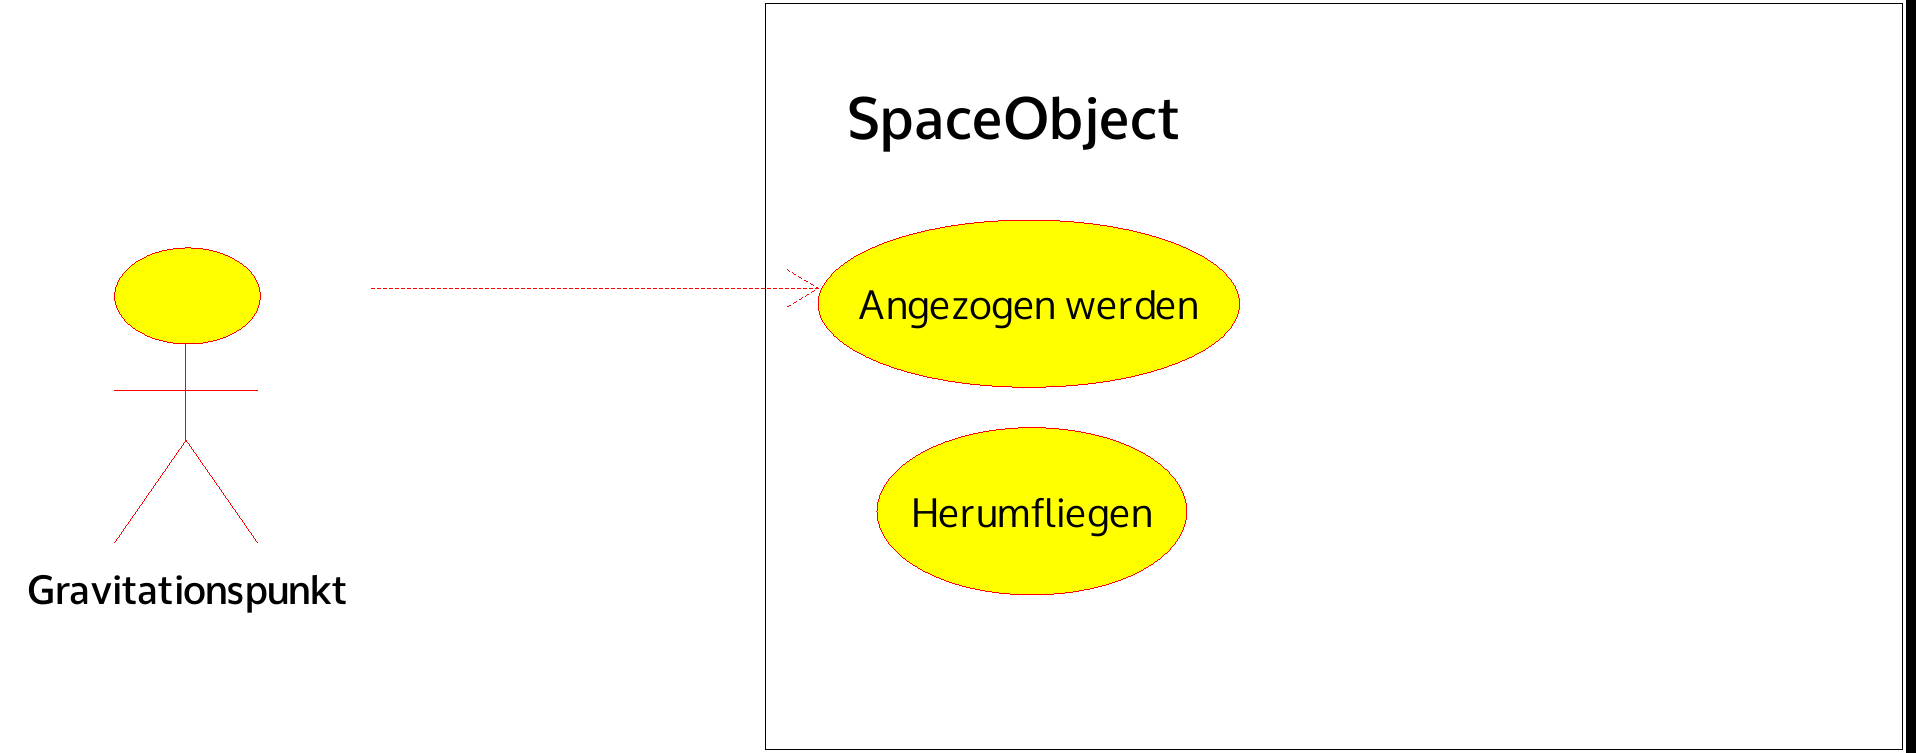
\includegraphics[scale=0.2]{use_cases/spaceObject.png}\\
Ein spaceObject kann von einem Actor (Gravitationspunkt) angezogen werden. Das spaceObject
\q{fliegt} aber jeder Zeit \q{herum}. Dazu braucht es keinen Actor.

\subsubsection{Spieler}
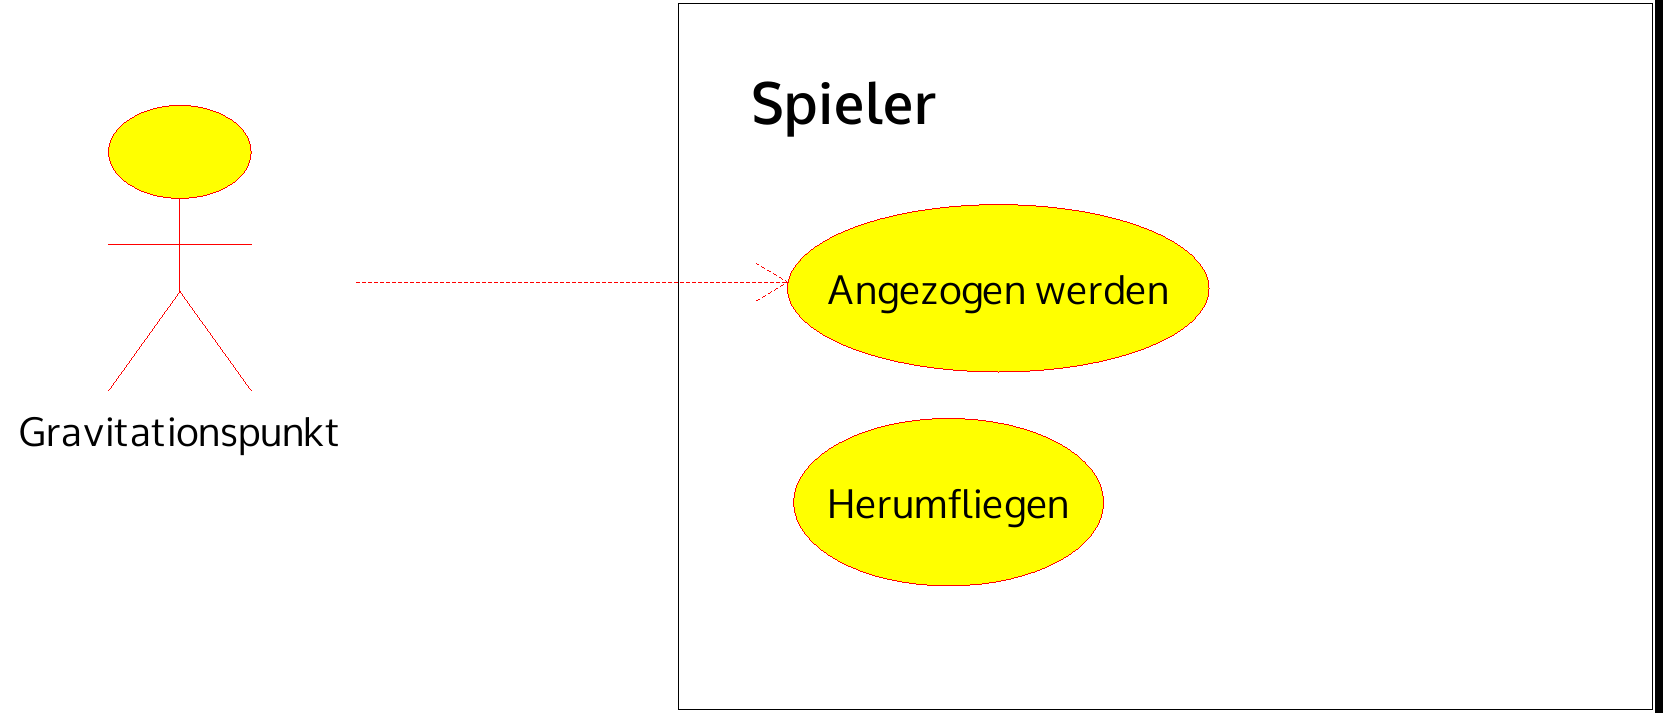
\includegraphics[scale=0.2]{use_cases/spieler.png}\\
Der Spieler kann, genau wie ein spaceObject von einem Gravitationspunkt angezogen werden. Unabhängig davon besitzt er seine eigenen
Geschwindigkeitsvektor, der seine Richtung bestimmt und nachdem er immer (und auch ohne Actor) fliegt.


\subsection{Anforderungen} 
\subsubsection{Technische Ausführung}
\begin{itemize}
\item Mit der Maus soll das Setzen eines Gravitationspunktes - und damit die Steuerung der Spielfigur - möglich sein.
\item Mit der Tastatur soll man aus dem Spiel zurück ins Menü gelangen. (Escape-Taste)
\item Das Spiel soll in ein eigenes Fenster registrieren, in das wir zeichnen können. 
\item Java packages: \begin{itemize}
	\item java.util.* \textit{(Native Java Datenstrukturen/Klassen, z. Bsp. Vector, Scanner)}
	\item java.io.* \textit{(Um Daten aus der .jar-Datei direkt als Streams zu lesen)}
\end{itemize}
\item JSFML packages: \begin{itemize}
	\item org.jsfml.graphics.* \textit{(Grafik-API von JSFML, für Sprites, Anzeige, etc.)}
	\item org.jsfml.system.* \textit{(System-API von JSFML, für Timer, etc.)}
	\item org.jsfml.window.* \textit{(Window-API von JSFML, für Fenster, Eingabe, etc.)}
\end{itemize}
\end{itemize}

\subsection{Dokumentation}
Diese Dokumentation wurde in \LaTeX \,\, erstellt. Da die Rohdateien in LaTeX im Textformat und nicht
binär vorliegen konnten wir sie ebenfalls in unser Revisionskontrollsystem einbinden und parallel
an ihr schreiben.\\

Da wir unseren Code mit den entsprechenden Kommentaren ausgeschmückt haben,
konnten wir eine detaillierte Codedokumentation mit dem Programm \textit{doxygen} (ähnlich wie javadoc) erstellen lassen.
Die PDF-Datei, die dabei herauskam liess sich leicht an unsere Dokumentation anhängen.\\

Der Quellcode wurde über das \textit{listings}-Paket direkt von LaTeX selbst eingelesen und formatiert.

\subsubsection{Technischer Ablauf des Spiels / spaceObjects}
Wie man in der Story zu unserem Spiel lesen kann, dreht sich unser Spiel vollständig um den Wissenschaftler im Raumschiff. Eigentlich geht es nur um das Raumschiff, denn dieses muss man sicher ans Ziel bringen.
Um dieses Raumschiff zu erstellen, nutzten wir die JSFML Bibliotheken.	\\

Zuerst erstellen, skalieren und positionieren wir das Fenster auf den Zeilen 234-236 der Klasse Game.java.
Danach erstellen wir eine View.
Solch eine View kann man sich als eine Kamera vorstellen, die mobil ist und nur das anzeigt, was sie sieht.
Zuerst ist diese View eine Standard-View und hat die Dimensionen des Fensters.
In Zeile 541 setzen wir jedoch diese Kamera auf den Spieler.
Damit überhaupt etwas angezeigt werden kann, muss es gezeichnet werden. 

Die Klasse \textit{RenderWindow} besitzt deshalb eine Methode \textit{draw(Drawable)}, die wir vor allem am Ende der Game-Klasse aufrufen.
Mit dieser Methode wird das bestimmte Objekt des Typs Drawable auf das Fenster gezeichnet.
Es gibt viele Klassen in den JSFML-Bibliotheken, die von dieser Klasse erben, sich also auf im Spielfenster zeichnen lassen.
Eine dieser Klassen nutzten wir jedoch am Häufigsten: Die Klasse \textit{jsfml.Graphics.Sprite}.		\\
Die JSFML-Klasse Sprite ist sehr nützlich für Objekte, die sich bewegen und laufend neu gezeichnet werden sollten.
Ein solches Sprite besteht einfach gesagt aus einer Texture (das Anzeigebild, bei unserem Spieler zum Beispiel das Bild des Raumschiffs) mit einem Rechteck,
welches oftmals die Dimensionen des Bides besitzt und die Positionsdaten dieser Figur speichert.

Unser Spieler besteht und wird ebenfalls durch ein solches Sprite visualisiert.
Da wir für unser Spiel noch mehr Informationen brauchen, als nur die Positionsdaten, die in einem
Sprite gespeichert werden (zum Beispiel die Geschwindigkeit, etc.), haben wir eine eigene Klasse für Objekte erstellt. Da sich diese Objekte
in unserem Spiel im Weltraum bewegen, haben wir die Klasse \textit{SpaceObject} benannt. Unser Spieler ist also ebenfalls ein spaceObject.

Die Sprite-Klasse wurde von den JSFML-Entwicklern \q{finalisiert}. Es war uns also nicht
möglich aus dieser Klasse eine neue Klasse zu be-erben.


Die Klasse SpaceObject brauchen wir sowohl für das Raumschiff wie auch für die Asteroiden.


Das ganze Spiel basiert auf einer while-Schleife, die in Game.java in Zeile 313 beginnt.
Diese Schleife läuft solange das Fenster offen bleibt weiter; dadurch realisieren wir ein ständiges Fortlaufen des Spieles.
Zum Beispiel wird die vorher beschriebene Methode draw(Drawable) innerhalb dieser Schleife ausgeführt.
So werden die Texturen ständig aktualisiert und sichergestellt, dass keine Veränderungen stattfinden, die nicht dargestellt werden.
Um nun den Spieler anzeigen zu lassen, rufen wir den Konstruktor der SpaceObjects auf und laden das Bild: 	\\

\begin{center}
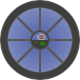
\includegraphics[scale=1]{img/spieler.png}
\end{center}

Danach lassen wir das Sprite des SpaceObjects zeichnen.




\subsubsection{Raum frei von auswärtigen Kräften}
Unser Spiel befindet sich irgendwo in einem fiktiven Weltraum. Es gibt keine grossen Körper um das
Level herum, die die Gravitation auf besondere Weise beeinflussen würden. Dies haben wir bewusst weggelassen.


\subsubsection{Gravitation}
Im Spiel finden sich sogenannte Gravitationspunkte, die den Spieler unterschiedlich stark anziehen.
Um diese Punkte zu implementieren, mussten wir uns durch etwas Physikliteratur wälzen und entsprechende
Anpassungen vornehmen, um die Gravitation mit vertretbarem Programmier- und auch Rechenaufwand implementieren zu können.  \\

Unsere Gravitation stellt eine vereinfachte Simulation dar, die nicht ganz mit der Realität übereinstimmt.
So ziehen sich in der echten Welt Objekte gleichzeitig an, was zu komplizierten gekoppelten Gleichungen führt, während dies in
unserem Spiel vernachlässigt wird und die Anziehungswirkung sequentiell in kleinen Abständen berechnet wird.\\

Alle Objekte, auf die sich die Gravitation im Spiel auswirken kann (sog. spaceObjects), befinden sich in einer Liste (\textit{spaceObjects})
In einer äusseren Schleife werden alle Objekte durchiteriert, in der inneren Schleife werden die Auswirkungen jedes Gravitationspunktes berechnet und
das Objekt verschoben. In Pseudocode:
\begin{verbatim}
FÜR jedes objekt in spaceObjects:
    FÜR jeden punkt in objekt.gravitationsPunkte:
        objekt.addEnergy(punkt.getEnergy(objekt))
\end{verbatim}

wobei \textit{auswirkungen} ein (mathematischer) Vektor ist, der \q{Energieänderungen} in $x$- und $y$-Richtung angibt.
Da dies den rechnerischen Teil der Gravitationspunkte betrifft, findet sich die Implementierung in der \textit{GravityModel}-Klasse
Wenn $m$ die Masse des spaceObjects ist, berechnet sich die Energieänderung wie folgt:
Seien $\Delta x$ und $\Delta y$ die Differenzen der Koordinaten zwischen dem spaceObject und dem Gravitationspunkt,
folglich ist $d = \sqrt{\Delta x^2 + \Delta y^2}$ der direkte Abstand. Die neue Energie eines Objektes (in $x$- und $y$-Richtung)
ist damit gegeben als (siehe \textit{gravityModel.getEnergy()}): 
\[ \vec{E}_{neu} = \vec{E} + m \cdot \frac{1}{d} \begin{pmatrix}\Delta x \\ \Delta y\end{pmatrix} \]

Aus dieser Energie lässt sich wiederum die neue Geschwindigkeit des Objekts berechnen (siehe \textit{spaceObject.updateVelocity()}):
\[ \vec{v}_{neu} = \frac{2}{m} \cdot \vec{E}_{neu}\] 

Die Formeln entsprechen ebenfalls nicht ganz der Realität, so wird in der klassischen Physik zwischen Beschleunigung, Energie und Kraft unterschieden,
während wir diese Begriffe etwas unsauber mischen. Die Kraft, mit der sich 2 Objekte - nach Newton - anziehen, beträgt
\[ F = G \cdot \frac{m_1 \cdot m_2}{d^2} \]
und nimmt im Abstand quadratisch ab. Unsere Tests ergaben aber, dass bei quadratisch abnehmender Gravitation, das
Spiel nicht mehr \q{so lustig} war, wie mit linearer Gravitation. Die Objekte wurden in einem gewissen Abstand, wie er
im Spiel durchaus vorkommen könnte, (fast) gar nicht angezogen, die Bahnkurven waren aber in der Nähe der Objekte
unberechenbar und das Spiel somit nicht wirklich spielbar. Deshalb entschieden wir uns, die Anziehungskraft
nur linear abzuschwächen lassen.


\subsubsection{Spieler bewegen / Gravitationspunkt}
Anders als bei anderen 2D-Spielen (SuperMario, Pacman, etc...) ist es in unserem Spiel nicht
möglich den Spieler per Pfeiltasten zu steuern. Es ist nur möglich einen Gravitationspunkt zu setzen, der den Spieler gegen sich zieht.
Da der Spieler nicht durch die Wände fliegen kann, prallt er daran ab und kommt nicht unbedingt zum Ziel. Es gilt also
die Gravitationspunkte so zu setzen, dass der Spieler damit bewusst in die richtige Richtung beschleunigt und gebremst werden kann.\\

Die Schwierigkeit besteht also darin, dass gezielte Bremsmanöver (zum Beispiel vor einem Asteroiden) fast nicht möglich sind und 
der Spieler trotzdem in der vorgesehenen Zeit durch das Level kommen soll.


\subsubsection{Levels}
Unser Ziel war es, ein System zu entwickeln, welches eine einfache Erstellung und Bearbeitung von Levels ermöglicht. Um dies zu erreichen, haben wir uns entschieden, die Levels in einem Tile-System aufzubauen. Damit ist gemeint, dass die Levels so aus \q{Tiles} (\textit{eng.} Kacheln, Fliesen) bestehen, wie ein Fliesenboden aus Fliesen besteht. So werden also vorerst einzelne Tiles erstellt und dann zu einem Level zusammengefügt.\\

\textbf{tileTypes}\\
Die tileTypes sind die verschiedenen Tiles, aus welchen das Level aufgebaut werden kann. Sie entsprechen beim Fliesenlegen also dem Sortiment an verschiedenen Fliesen. tileTypes können verschiedene Hintergrundtexturen, spaceObjects, gravityObjects und blackHoles haben. All diese Eigenschaften werden in TileType-Dateien gespeichert. TileType-Dateien sind normale Textdateien, die folgendermassen aufgebaut sind:\\
\begin{tabular}{ | r | r | l | }
	\hline
	\multicolumn{2}{ | r | }{\textbf{Datentyp}} & \textbf{Inhalt}\\ \hline
	\multicolumn{2}{ | r | }{int} & hintergrundId\\ \hline
	\multicolumn{2}{ | r | }{int} & anzahlSpaceObjects\\ \hline
	 & string & texturePfad\\ \cline{2-3}
	 & float &	m\\ \cline{2-3}
	 & floats & EX, EY\\ \cline{2-3}
	 & floats & posX, posY\\ \cline{2-3}
	 & boolean	& gravityOn\\ \hline
	\multicolumn{2}{ | r | }{int} & anzahlGravityFields\\ \hline
	 & floats & posX, posX\\ \cline{2-3}
	 & float & m\\ \hline
	\multicolumn{2}{ | r | }{int} & anzahlBlackHoles\\ \hline
	 & float & m\\ \hline
\end{tabular} \\
Jede Zeile der Tabelle entspricht einer Zeile in einer TileType-Datei, wobei die eingezogenen Zeilen pro spaceObject bzw. gravityField oder blackHole einmal vorkommen. Jeder tileType hat eine Identifikationsnummer. Diese wird im Namen der TileType-Datei angegeben. So hat also der tileType, dessen TileType-Datei den Namen \q{tile1} trägt die Identifikationsnummer 1.\\

\textbf{Levels}\\
Die einzelnen Tiles werden dann in der Level-Datei \q{zusammengesetzt}. Eine Level-Datei ist wie folgt aufgebaut:\\
\begin{tabular}{ | r | r | l | }
	\hline
	\multicolumn{2}{ | r | }{\textbf{Datentyp}} & \textbf{Inhalt}\\ \hline
	\multicolumn{2}{ | r | }{int} & levelTimeAvailable\\ \hline
	\multicolumn{2}{ | r | }{floats} & startX, startY\\ \hline
	\multicolumn{2}{ | r | }{floats} & zielX, zielY\\ \hline
	\multicolumn{2}{ | r | }{ints} & width, height\\ \hline
	 & ints & id1, id2, id3, id4,\dots\\ \cline{2-3}
	 & ints & id1, id2, id3, id4,\dots\\ \cline{2-3}
	 & \dots & \dots\\ \hline
\end{tabular}\\
Erneut entspricht jede Zeile der Tabelle einer Zeile in der Level-Datei. Hierbei entspricht die Anzahl Zeilen im Format der eingezogenen Zeilen in der Level-Datei dem Wert \textit{height} und die Anzahl Ganzzahlen pro Zeile dem Wert \textit{width}. Die Ganzzahlen \textit{id1, id2, id3, id4,\dots} sind die Identifikationsnummern der tileTypes, welche an jener Stelle als Tile \\

\textbf{Level-Klasse}\\
Der Konstruktor der Level-Klasse hat die Aufgabe, eine Level-Datei zu lesen und dann anhand der TileType-Dateien ein Level-Objekt zu kreieren, welches alle für ein Level nötige Objekte enthält. So hat ein Level-Objekt jeweils einen Vektor mit allen spaceObjecs, gravityFields, blackHoles und zusätzlichen Sprites, die im Level erscheinen sollten. Auch weitere Variabeln, wie die verfügbare Zeit, Start-Koordinaten und Koordinaten des Ziels, sowie die Anzahl Tiles in der Breite und in der Höhe des Levels sind in einem Level-Objekt enthalten.\\
Um all dies aus einer Level-Datei und aus den TileType-Dateien zu lesen wird ein Scanner kreiert, der die Level-Datei öffnet. Der Scanner Wert für Wert durch die Datei und Speichert die gelesenen Werte in den entsprechenden Variabeln.  Wenn er bei den Identifikationsnummern der tileTypes ankommt, ruft er die Methode \textit{loadTile} mit der Identifikationsnummer als tileType auf, welche dann mit einem eigenen Scanner die entsprechende TileType-Datei öffnet und anhand der daraus gelesenen Informationen die nötigen Objekte erstellt.


\textbf{Start und Ziel}
\\
\todo{Hier vervollständigen}
\textbf{Wände}

\subsubsection{- Gegner und Hindernisse}
% Asteroiden und Schwarzes Loch

Nebem dem Spieler haben wir zwei weitere Objekte erschaffen.
Zum einen sind das die Asteroiden, andererseits sind das die Schwarzen Löcher.		\\

\textbf{Asteroiden}		\\
Die Asteroiden sind wie der Spieler Objekte

\textbf{Schwarze Löcher}		\\
...


\subsubsection{Gameover}
Wenn der Spieler mit einem Asteroiden kollidiert oder in ein schwarzes Loch
hineingezogen wird, ist das Spiel vorbei. Wird festgestellt, dass sich die 
Positionen des Spielers und eines anderen Objektes überschneiden, wird eine boolsche
Variable $gameOver$, die beim Start mit $false$ initialisiert wurde, auf $true$ gesetzt.

Vor dem eigentlich Rendering, also wenn alle Änderungen der Spielewelt berechnet wurden
und nur noch alles auf den Bildschirm gezeichnet werden muss, wird auf dieses Flag getestet.
Kollidierte der Spieler also seit dem letzten Rendervorgang, werden nicht mehr alle Objekte
gezeichnet, sondern nur eine Grafik die sich mit \q{GAME OVER} über den Spielbildschirm erstreckt.

Mit der Escape-Taste gelangt man dann wieder zurück ins Hauptmenü. Wird ein neues Level geladen,
wird die $gameOver$-Variable wieder auf $false$ gesetzt, damit das Spiel starten kann.


\subsubsection{Kleine Reibung}
Wenn ein Objekt angezogen wird, ihm somit Energie hinzugefügt wird, wird die neue Energie des Objekts auf 99\%
des ursprünglichen Wertes gesetzt. (Siehe \textit{spaceObjectModel.addEnergy()}) Bei genug einzelnen Schritten konvergiert damit die Energie des Objekts gegen 0 und
das Objekt pendelt sich am Gravitationspunkt ein. Dies haben wir so implementiert, damit es für den Spieler leicht ist,
sein Raumschiff an einer bestimmten Stelle zu fixieren.
\[ \vec{E} = \vec{E}_{alt} \cdot 0.99 \]
\[ \lim_{n\rightarrow \infty} \vec{E} \cdot 0.99^n = \begin{pmatrix}0\\0\end{pmatrix} \] 

\subsubsection{Zeit}
Beim Laden des Levels wird ein Zähler gestartet. Jedes Level besitzt sein eigenes Zeitlimit, das in der Leveldatei frei wählbar ist.
Diese Zeit wird dem Spieler nicht angezeigt. Verstreicht diese Zeit und der Spieler schafft es unterdessen nicht an das Ziel des Levels,
hat der Spieler ebenfalls verloren und die Gameover-Grafik wird angezeigt.

\subsubsection{Startmenü}
Das Startmenü zeigt ein Hintergrundbild und zwei Buttons (die über Sprites visualisiert werden), die dazu dienen das Spiel zu starten oder es zu beenden.
Wenn das Menü angezeigt wird, wird eine Liste aller verfügbaren Levels aus der .jar-Datei gelesen. Es wird dann eine
Liste aller Level im Startmenü angezeigt, sodass man direkt das Level, welches man durchspielen möchte, wählen kann.
Ob und welcher Button/Level angeklickt wurde wird mithilfe der Positionen der Button- bzw. der Textkoordinaten überprüft.
Bei einem Klick wird anschliessend das Level geladen und das Flag, das das Menü sichtbar macht (\textit{menuAktiv}) auf $false$
gesetzt. Somit wird das Level sicht- und spielbar. Drückt der Spieler Escape wird automatisch das Flag \textit{menuAktiv} wieder auf $true$
gesetzt und der Spieler gelangt vor dem nächsten Renderzyklus wieder in das Hauptmenü.

\subsubsection{Spielanleitung}
\inmilestonetwo

\clearpage
\newpage
\section{Entwurf}
\subsection{UML Diagramm}
\vspace{0.3cm}
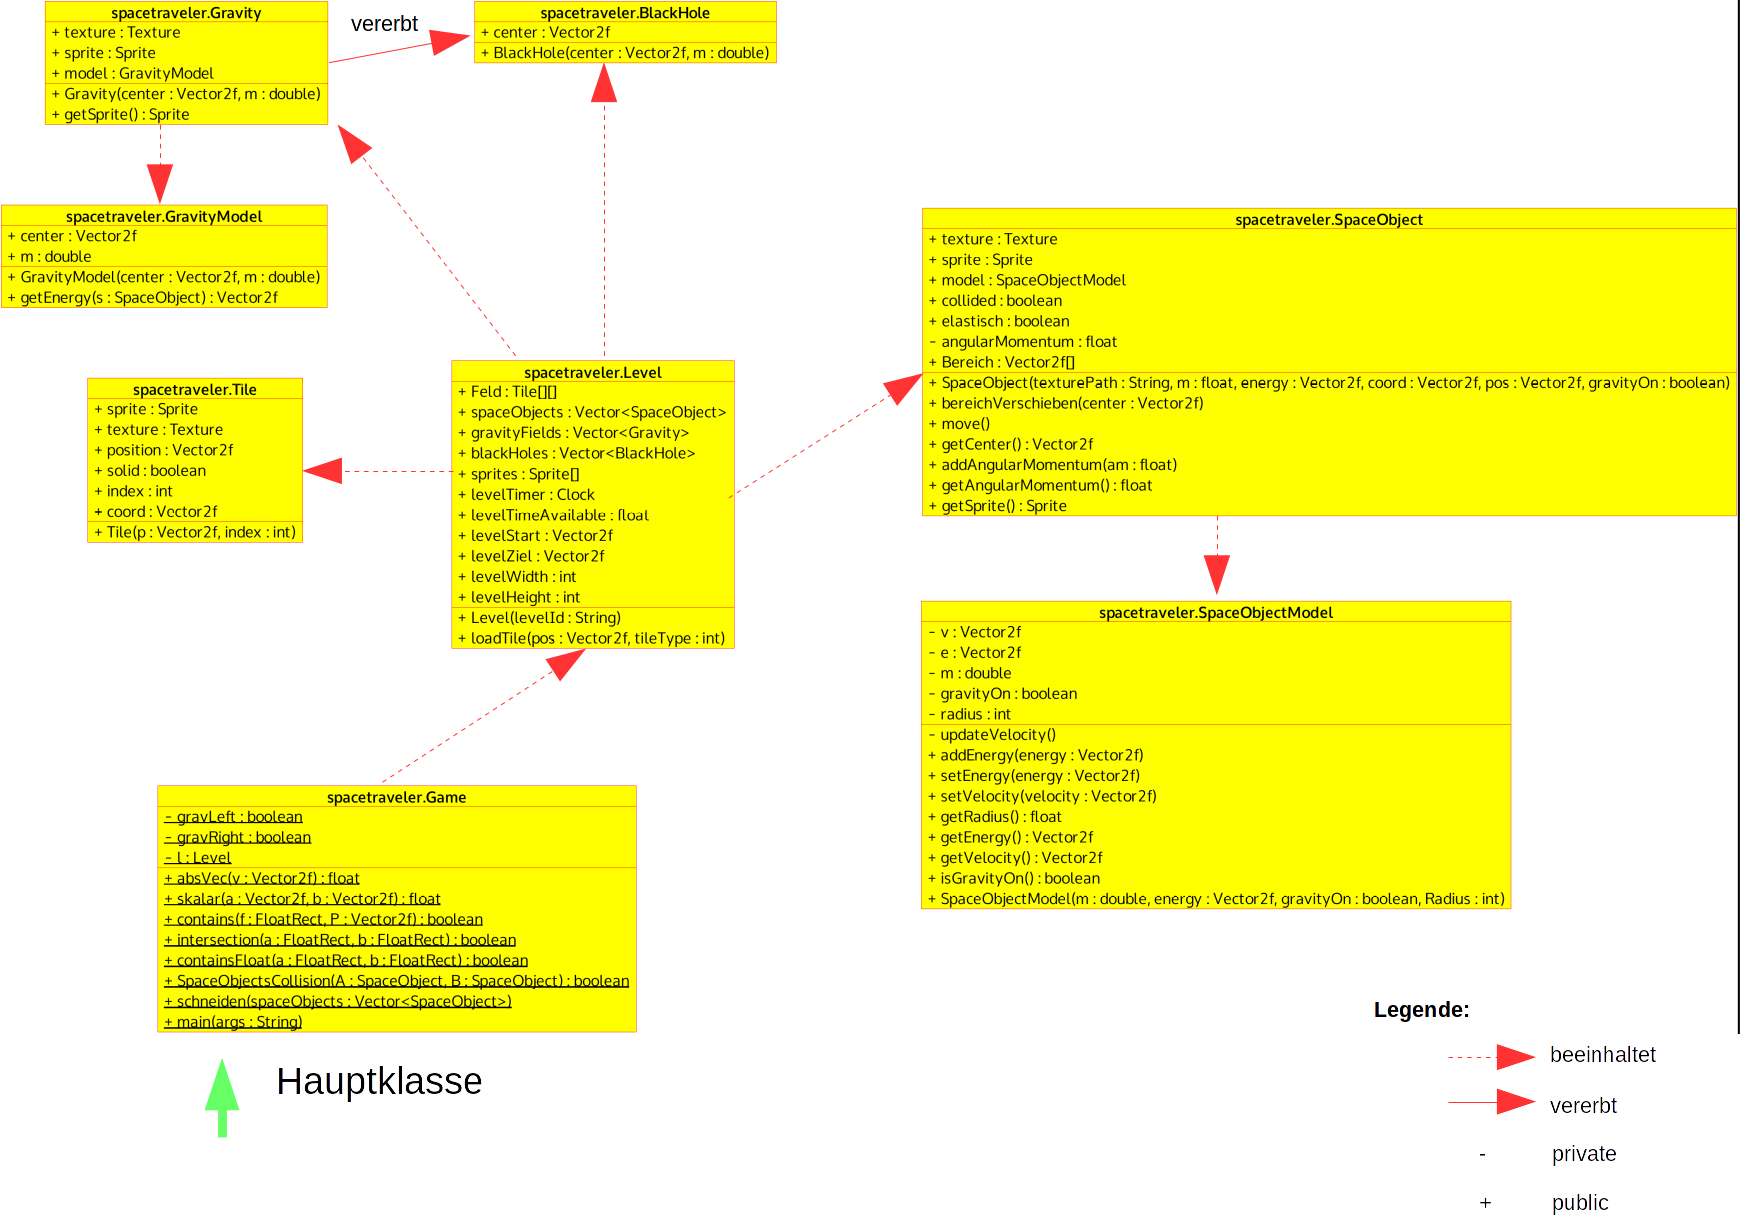
\includegraphics[height=0.85\textwidth,angle=90]{img/uml.png}

\section{Implementierung}
% Quellcode
\section{Quellcode}
\subsection{Über unseren Quellcode}
Unser Code ist modular aufgebaut, d.h. das Spiel besteht aus verschiedenen Klassen. Jede Klasse
verfügt über eine eigene Datei.
\subsection{Level.java}
\lstinputlisting[language=Java,breaklines=true,numbers=left,tabsize=4]{../../src/spacetraveler/Level.java}
\fontsize{12pt}{14pt}\selectfont

\section{Resultate und Testen}
\inmilestonetwo
\section{Diskussion und Ausblick}
\inmilestonetwo


\section*{Anhang: Codedokumentation}
In unserem Code haben wir Kommentare zu den einzelnen Klassen und Methoden hinzugefügt.
Diese Kommentare werden vom Programm \textit{doxygen} automatisch extrahiert und es wird eine
Dokumentation aller Klassen und Methoden erstellt. In der Dokumentation finden sich auch
Grafiken. Diese Dokumentation folgt hier im Anhang:\\

%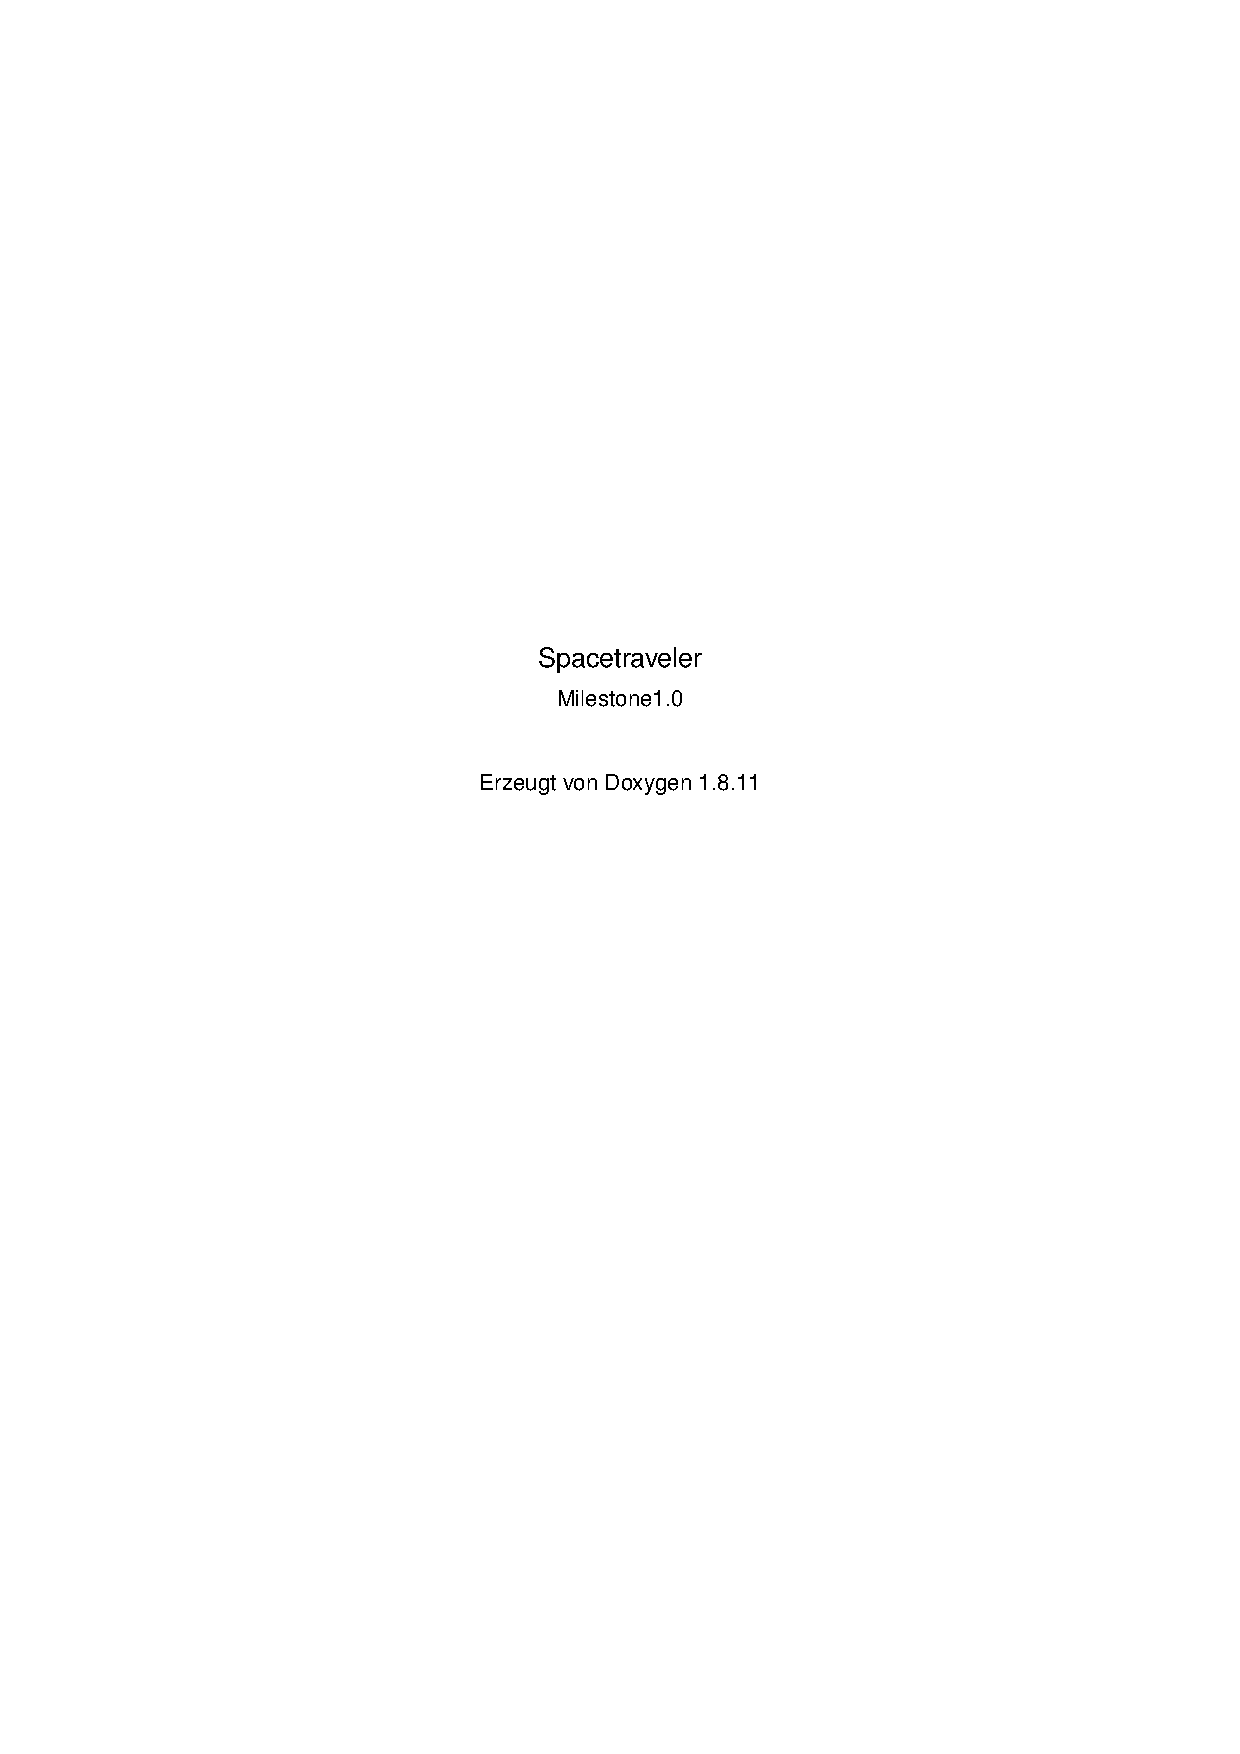
\includepdf[pages=-]{refman.pdf}

\ 


\end{document}
 
